\documentclass[12pt]{article}
\usepackage[margin=2.5cm]{geometry}
\usepackage{enumerate}
\usepackage{amsfonts}
\usepackage{amsmath}
\usepackage{fancyhdr}
\usepackage{amsmath}
\usepackage{amssymb}
\usepackage{amsthm}
\usepackage{mdframed}
\usepackage{graphicx}
\usepackage{subcaption}
\usepackage{adjustbox}
\usepackage{listings}
\usepackage{xcolor}
\usepackage{booktabs}
\usepackage[utf]{kotex}
\usepackage{hyperref}
\usepackage{accents}

\definecolor{codegreen}{rgb}{0,0.6,0}
\definecolor{codegray}{rgb}{0.5,0.5,0.5}
\definecolor{codepurple}{rgb}{0.58,0,0.82}
\definecolor{backcolour}{rgb}{0.95,0.95,0.92}

\lstdefinestyle{mystyle}{
    backgroundcolor=\color{backcolour},
    commentstyle=\color{codegreen},
    keywordstyle=\color{magenta},
    numberstyle=\tiny\color{codegray},
    stringstyle=\color{codepurple},
    basicstyle=\ttfamily\footnotesize,
    breakatwhitespace=false,
    breaklines=true,
    captionpos=b,
    keepspaces=true,
    numbers=left,
    numbersep=5pt,
    showspaces=false,
    showstringspaces=false,
    showtabs=false,
    tabsize=1
}

\lstset{style=mystyle}

\pagestyle{fancy}
\renewcommand{\headrulewidth}{0.4pt}
\lhead{CSC 343}
\rhead{Worksheet 9 Solution}

\begin{document}
\title{CSC343 Worksheet 9 Solution}
\maketitle

\bigskip

\begin{enumerate}[1.]
    \item \textbf{Exercise 11.1.1:}

    \bigskip

    \begin{enumerate}[a)]
        \item

    \begin{center}
    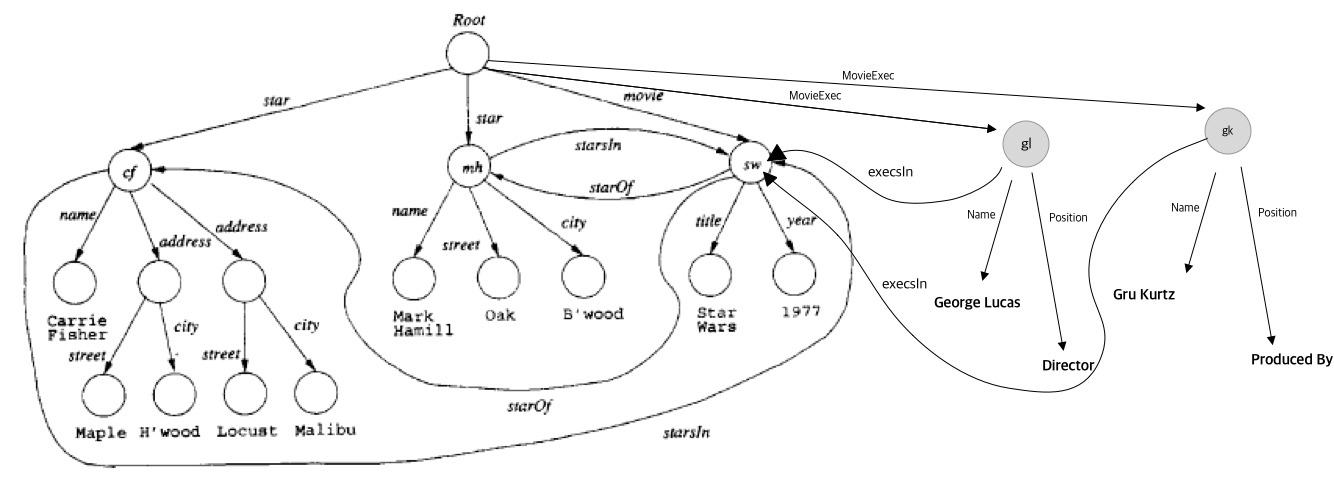
\includegraphics[width=\linewidth]{images/worksheet_9_solution_4.png}
    \end{center}

        \bigskip

        \underline{\textbf{Notes:}}

        \begin{itemize}
            \item Semistructured data
            \begin{itemize}
                \item serves as a model suitable for \textbf{databases integration}, that is,
                for describing the data contained in two or more databases that contain similar data with
                different schemas

                \item It serves as the underlying model for notations such as XML, to be taken
                up in Section 2, that are being used to share information on the web.
            \end{itemize}

            \item Semistructured Data Representation
            \begin{itemize}
                \item is a collection of nodes

            \begin{center}
            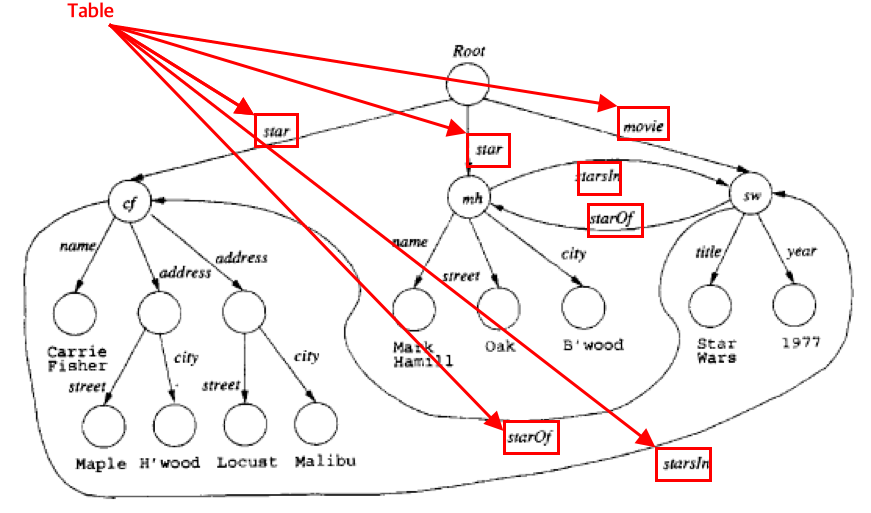
\includegraphics[width=\linewidth]{images/worksheet_9_solution_1.png}
            \end{center}

            \begin{center}
            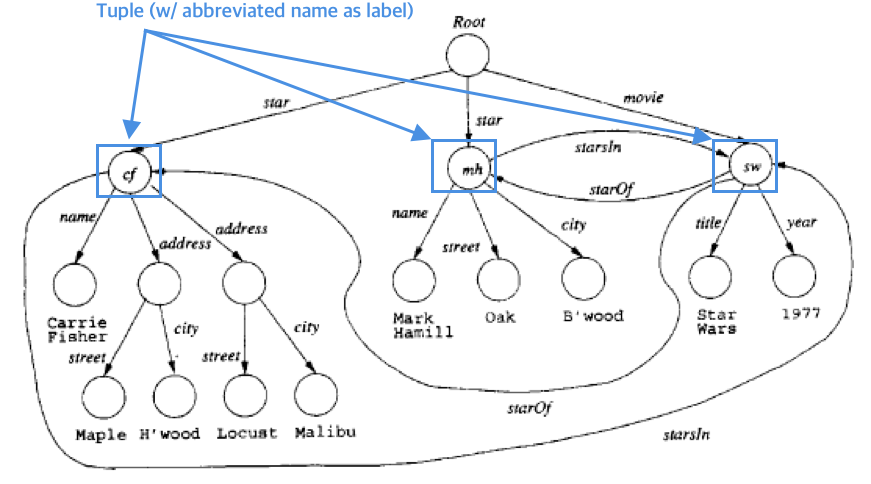
\includegraphics[width=\linewidth]{images/worksheet_9_solution_2.png}
            \end{center}

            \begin{center}
            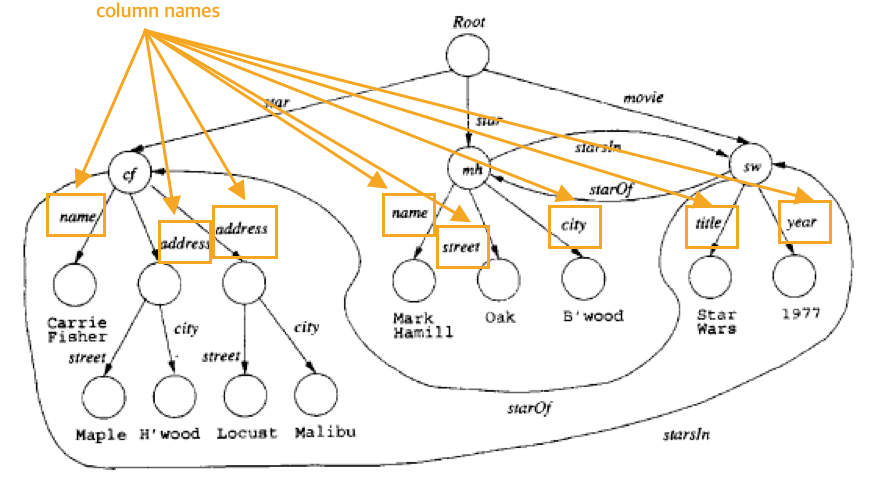
\includegraphics[width=\linewidth]{images/worksheet_9_solution_3.png}
            \end{center}

            \end{itemize}

            \item
        \end{itemize}

        \item

    \begin{center}
    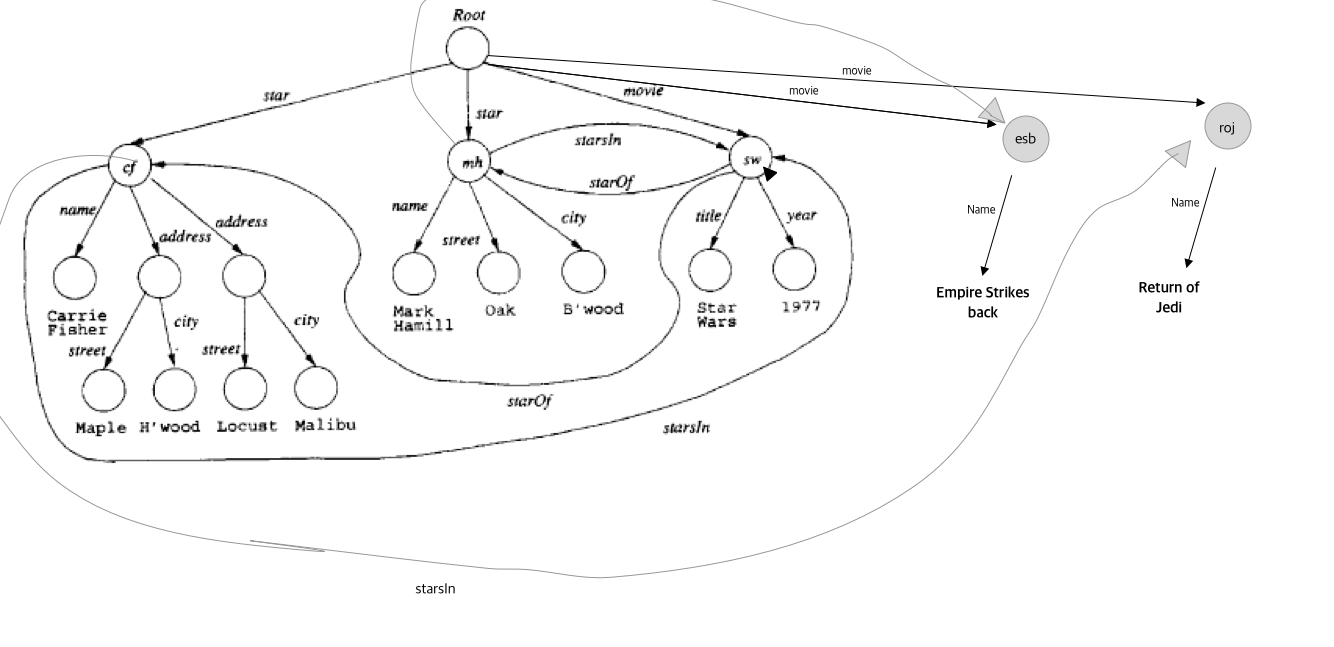
\includegraphics[width=\linewidth]{images/worksheet_9_solution_5.png}
    \end{center}


        \item

    \begin{center}
    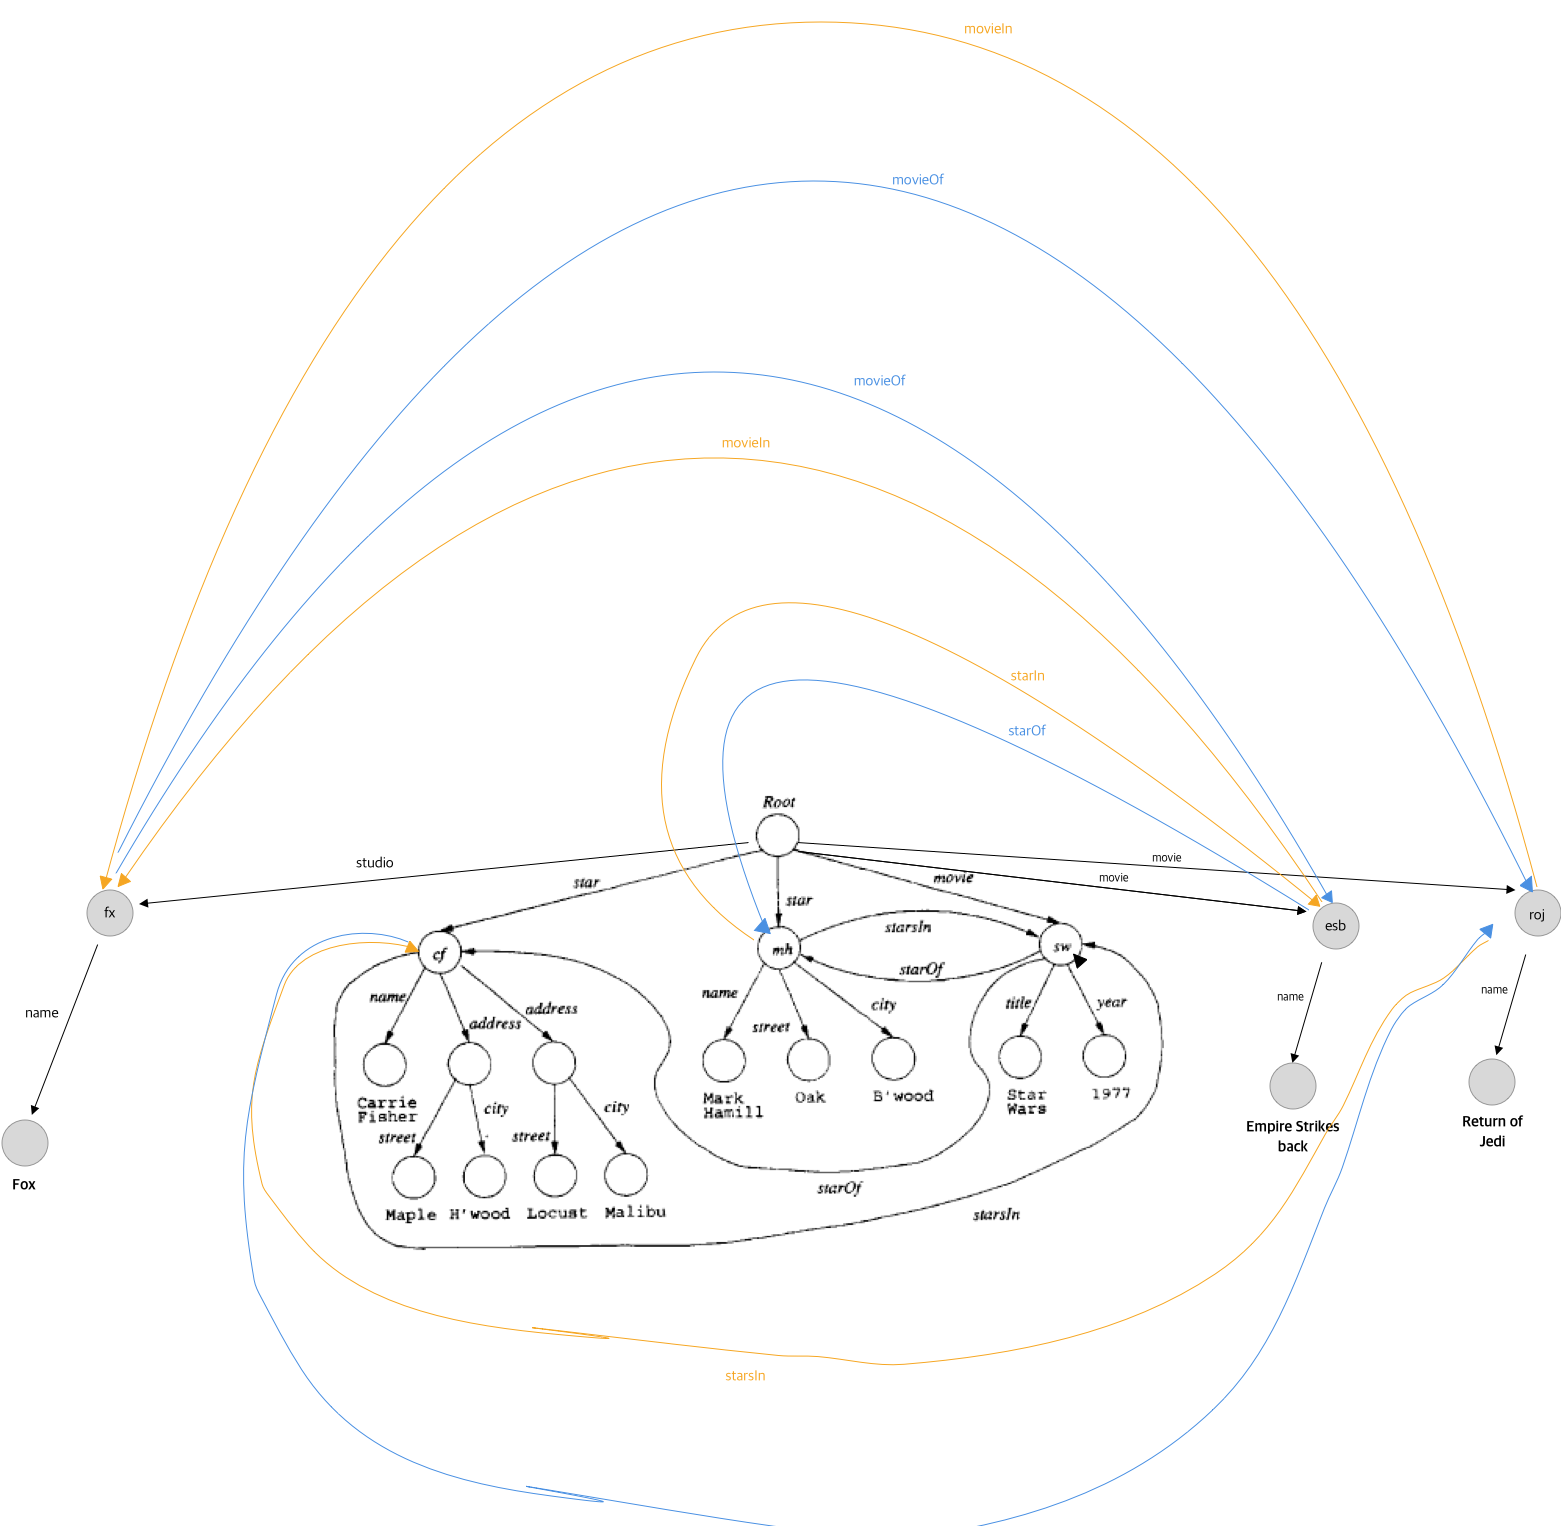
\includegraphics[width=\linewidth]{images/worksheet_9_solution_6.png}
    \end{center}

    \end{enumerate}

    \item

    \begin{center}
    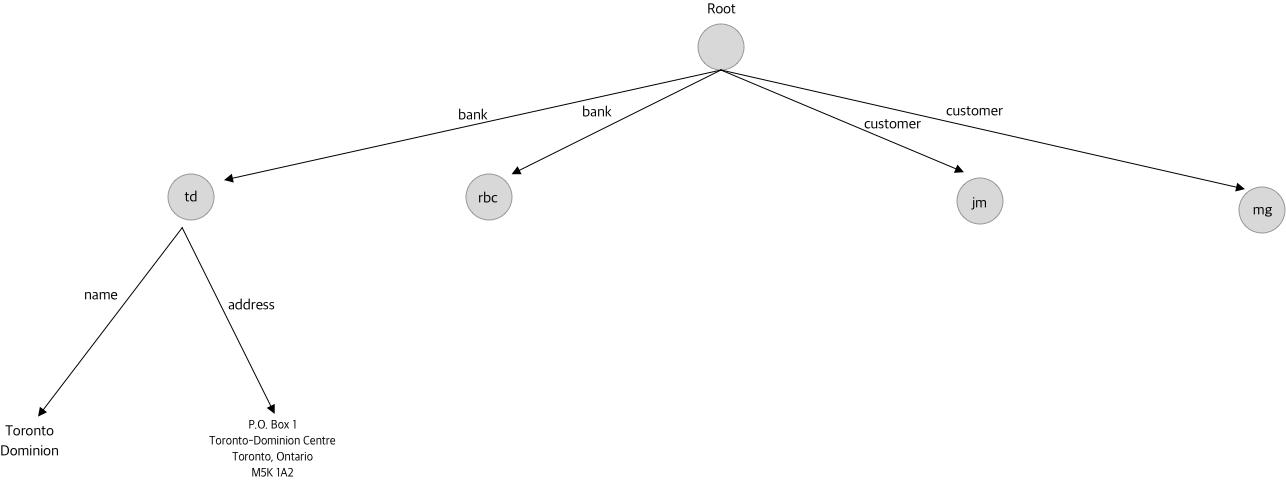
\includegraphics[width=\linewidth]{images/worksheet_9_solution_7.png}
    \end{center}


\end{enumerate}

\end{document}